\documentclass[11pt,a4paper]{article}
\usepackage[utf8]{inputenc}
\usepackage{amsmath, amsthm, amssymb}
\usepackage{graphicx}
\usepackage{float}
\usepackage{geometry}
\usepackage{hyperref}
\usepackage{booktabs}
\usepackage{caption}
\usepackage{subcaption}
\usepackage{xcolor}
\usepackage{ifthen}
\usepackage{ifpdf}

\geometry{margin=1in}

\newcommand{\figorp}[2]{%
  \IfFileExists{#1}{\includegraphics[#2]{#1}}%
  {\begin{center}\textit{[Run \texttt{Master\_Validation.m} to generate figure]}\end{center}}}

\title{\Large Kinematic Analysis and Trajectory Execution\\[4pt]
       of the KUKA LBR MED Surgical Manipulator\\[6pt]
       \large Phase~I \& Phase~II Report\\
       Robotic Systems in Manipulation 2025/2026}
\author{Instituto Superior T\'{e}cnico}
\date{Phase~I due: 17 May 2026 \qquad Phase~II due: 7 June 2026}

\begin{document}
\maketitle
\noindent\textbf{Professors:} Prof.\ Jorge Martins, Prof.\ Rui Coelho
\tableofcontents
\newpage

%% =========================================================
\section{Denavit--Hartenberg Convention}
%% =========================================================

\subsection{Robot Description}
The KUKA LBR Med 7 R800 is a 7-DOF redundant surgical manipulator
with all revolute joints. Its kinematic structure consists of alternating
perpendicular joint axes, giving one degree of intrinsic redundancy over
the 6-DOF task space.

\begin{table}[H]
  \centering
  \caption{Link dimensions.}
  \begin{tabular}{lll}
    \toprule
    Parameter & Value & Description \\
    \midrule
    $d_1$ & 0.340\,m & Base platform to shoulder (joint 2 axis) \\
    $d_3$ & 0.400\,m & Shoulder to elbow (joint 4 axis) \\
    $d_5$ & 0.400\,m & Elbow to wrist centre (joint 6 axis) \\
    $d_7$ & 0.126\,m & Wrist centre to flange \\
    \bottomrule
  \end{tabular}
\end{table}

\subsection{Frame Assignment (Standard DH Convention)}
Following the standard DH procedure:
\begin{enumerate}
  \item Number joint axes $z_0,\dots,z_6$ where $z_i$ is the axis of joint $i{+}1$.
  \item Place Frame~0 at the base with $z_0$ pointing vertically upward.
  \item For $i=1,\dots,6$, place $O_i$ at the intersection of $z_{i-1}$ and $z_i$.
  \item Define $x_i$ along the common normal from $z_{i-1}$ to $z_i$.
  \item Define $y_i$ to complete the right-handed frame.
  \item Place Frame~7 at the end-effector with $z_7\!\parallel\! z_6$ and $O_7$ at the flange centre.
\end{enumerate}
\textbf{Key structural observation:} all consecutive joint axes intersect,
so all link offsets satisfy $a_i=0$.

\begin{figure}[H]
  \centering
  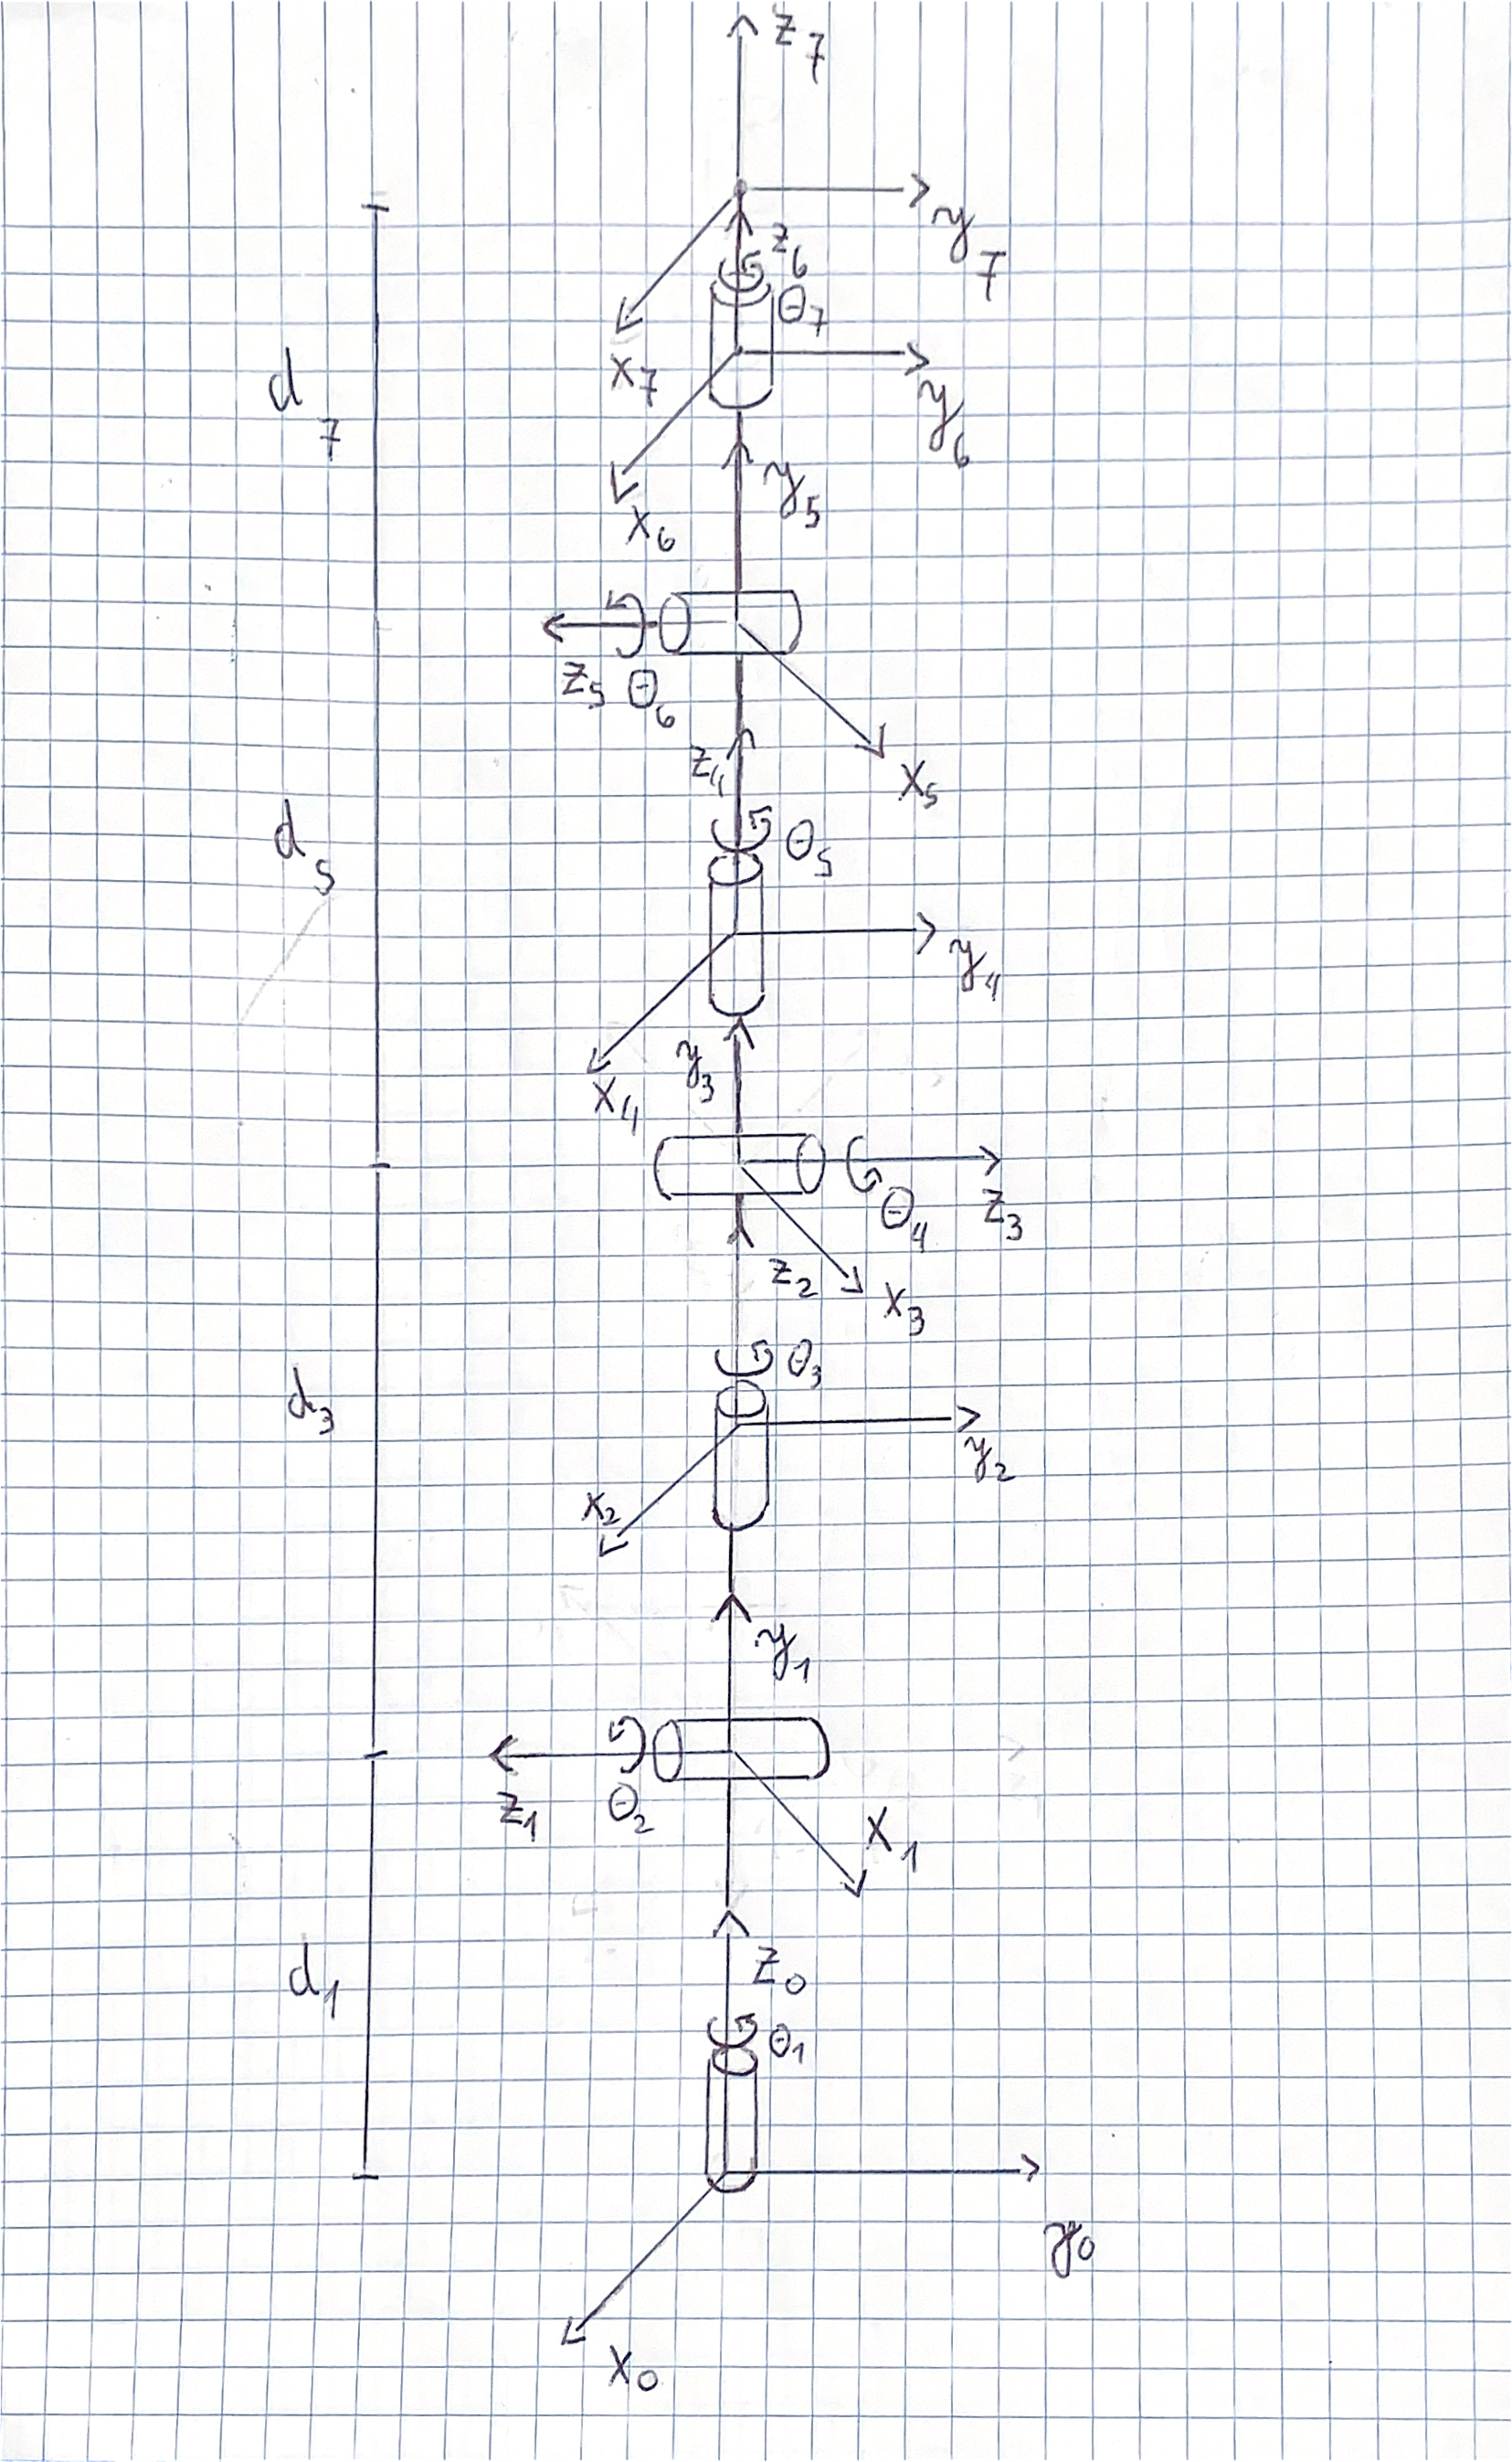
\includegraphics[width=0.78\textwidth]{dh-diagram.pdf}
  \caption{Hand-drawn DH frame assignment of the KUKA LBR MED.}
  \label{fig:dh_drawing}
\end{figure}

\subsection{DH Parameter Table}
The homogeneous transformation per link is:
\begin{equation}
  A_{i}^{i-1}(q_i) = R_z(\theta_i)\,T_z(d_i)\,T_x(a_i)\,R_x(\alpha_i)
\end{equation}

\begin{table}[H]
  \centering
  \caption{Standard DH parameters for the KUKA LBR MED.}
  \begin{tabular}{cccccl}
    \toprule
    Link $i$ & $a_i$ (m) & $\alpha_i$ (rad) & $d_i$ (m) & $\theta_i$ & Joint \\
    \midrule
    1 & 0 & $+\pi/2$ & 0.340 & $q_1$ & Base rotation \\
    2 & 0 & $-\pi/2$ & 0     & $q_2$ & Shoulder tilt \\
    3 & 0 & $-\pi/2$ & 0.400 & $q_3$ & Upper-arm rotation \\
    4 & 0 & $+\pi/2$ & 0     & $q_4$ & Elbow tilt \\
    5 & 0 & $+\pi/2$ & 0.400 & $q_5$ & Forearm rotation \\
    6 & 0 & $-\pi/2$ & 0     & $q_6$ & Wrist tilt \\
    7 & 0 & 0        & 0.126 & $q_7$ & End-effector rotation \\
    \bottomrule
  \end{tabular}
  \label{tab:dh_table}
\end{table}

%% =========================================================
\section{Direct Kinematics}
%% =========================================================

\subsection{Method}
Using the Symbolic Robotics MATLAB Toolbox, the direct kinematics
transformation is the ordered product of link matrices:
\begin{equation}
  T_7^0(q) = A_1^0(q_1)\,A_2^1(q_2)\,\cdots\,A_7^6(q_7)
\end{equation}
The position $p$ and rotation matrix $R$ of the end-effector in the base frame
are extracted from $T_7^0$ as its upper-left $3\times3$ block and upper-right
$3\times1$ column, respectively.

\subsection{Simulink Model}
\begin{figure}[H]
  \centering
  \begin{subfigure}[b]{0.35\textwidth}
    \centering
    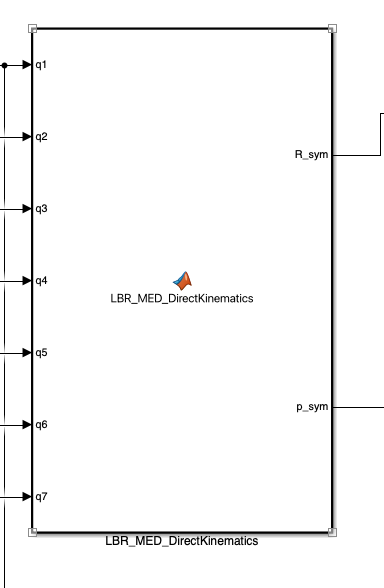
\includegraphics[width=\textwidth]{dkin-block.png}
    \caption{LBR\_MED\_DKin block.}
  \end{subfigure}
  \hfill
  \begin{subfigure}[b]{0.60\textwidth}
    \centering
    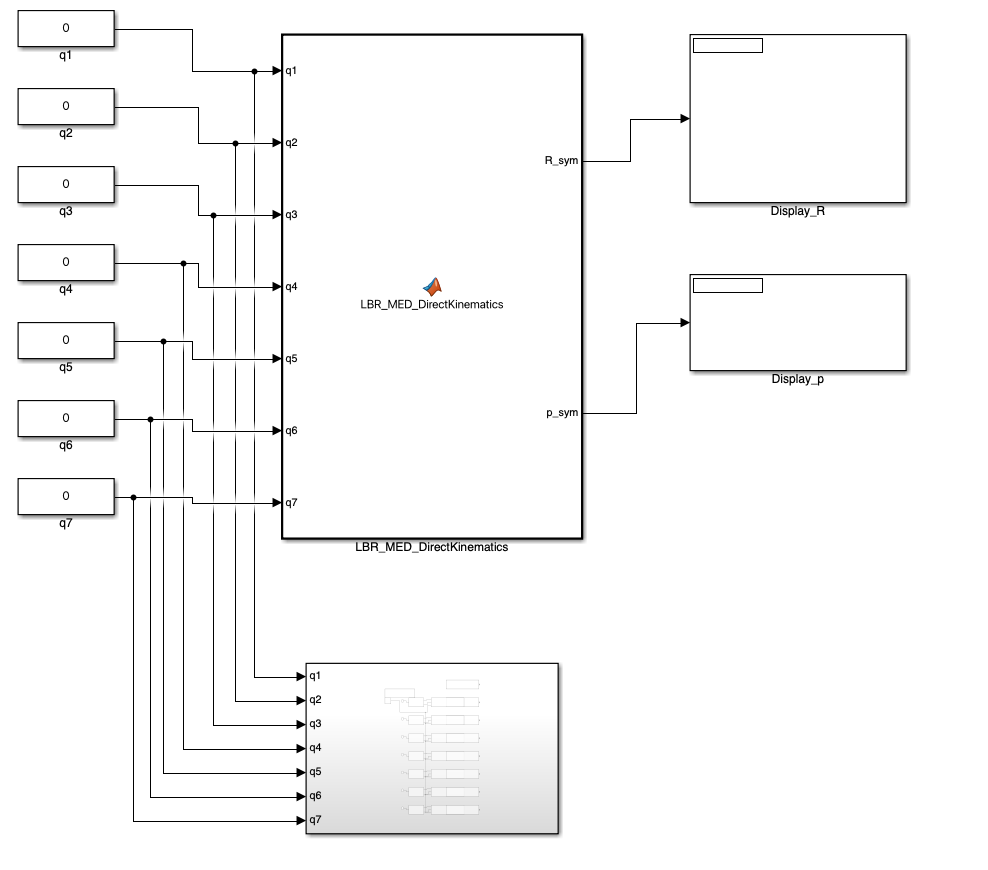
\includegraphics[width=\textwidth]{Dkin-simulink.png}
    \caption{Full validation model.}
  \end{subfigure}
  \caption{Direct kinematics Simulink model (LBR\_MED\_Simul.slx).}
  \label{fig:dkin_simulink}
\end{figure}

\subsection{Validation}
Four configurations are chosen where the end-effector pose can be
verified by geometric reasoning alone.

\begin{table}[H]
  \centering
  \caption{Direct kinematics validation results.}
  \resizebox{\textwidth}{!}{
  \begin{tabular}{lllll}
    \toprule
    Config & $q$ (rad) & Expected $p$ (m) & Expected $R$ & $\|p_{\mathrm{err}}\|$ \\
    \midrule
    1: Home          & all $= 0$                       & $[0,\;0,\;1.266]^\top$        & $I_3$         & $<10^{-12}$ \\
    2: Shoulder bend & $q_2=\pi/2$, rest $=0$          & $[-0.926,\;0,\;0.340]^\top$   & $R_y(-\pi/2)$ & $<10^{-12}$ \\
    3: Base spin     & $q_1=\pi/2$, rest $=0$          & $[0,\;0,\;1.266]^\top$        & $R_z(\pi/2)$  & $<10^{-12}$ \\
    4: Elbow fold    & $q_2=q_4=\pi/2$, rest $=0$      & $[-0.400,\;0,\;0.866]^\top$   & $I_3$         & $<10^{-12}$ \\
    \bottomrule
  \end{tabular}}
  \label{tab:dkin_val}
\end{table}

All four configurations pass with machine-precision errors, confirming
the symbolic DH product and the MATLAB function handles are correct.

%% =========================================================
\section{Inverse Kinematics (Closed-Form)}
%% =========================================================

\subsection{Kinematic Decoupling}
The robot has a spherical wrist (joints 5--7, axes $z_4$, $z_5$, $z_6$
intersecting at $O_6$), enabling the classical decoupling:
\begin{itemize}
  \item \textbf{Arm problem} (joints 1--4): position the wrist centre $O_6$.
  \item \textbf{Wrist problem} (joints 5--7): orient the end-effector.
\end{itemize}
\textbf{Redundancy resolution:} fixing $q_3=0$ reduces the arm to three
unknowns $(q_1,q_2,q_4)$ and yields a unique closed-form solution per branch.

\subsection{Closed-Form Solution}

\subsubsection*{Step 1 — Wrist centre}
\begin{equation}
  p_W = p_e - d_7\,a_e, \qquad a_e = R_d[:,3]
\end{equation}

\subsubsection*{Step 2 — Base rotation $q_1$}
\begin{equation}
  q_1 = \operatorname{atan2}(p_{Wy},\;p_{Wx})
  \quad\text{or}\quad q_1+\pi\ (\text{back-arm branch})
\end{equation}

\subsubsection*{Step 3 — Elbow angle $q_4$ (law of cosines)}
With $X=p_{Wx}\cos q_1+p_{Wy}\sin q_1$ and $Z=p_{Wz}-d_1$:
\begin{equation}
  \cos q_4 = \frac{X^2+Z^2-d_3^2-d_5^2}{2d_3d_5},
  \qquad \sin q_4 = \pm\sqrt{1-\cos^2 q_4}
\end{equation}

\subsubsection*{Step 4 — Shoulder angle $q_2$}
\begin{equation}
  \begin{bmatrix}-(d_3+d_5c_4)&d_5s_4\\d_5s_4&d_3+d_5c_4\end{bmatrix}
  \begin{bmatrix}s_2\\c_2\end{bmatrix}=\begin{bmatrix}X\\Z\end{bmatrix}
  \;\Rightarrow\; q_2 = \operatorname{atan2}(s_2,c_2)
\end{equation}

\subsubsection*{Steps 5--7 — Wrist angles $q_5,q_6,q_7$}
\begin{equation}
  R_{47}=\bigl(R_0^4\bigr)^\top R_d
\end{equation}
Reading off entries of the product $A_5A_6A_7$:
\begin{align}
  q_6 &= \operatorname{atan2}\!\left(\sqrt{1-R_{47}(3,3)^2},\;R_{47}(3,3)\right)\\
  q_5 &= \operatorname{atan2}\!\left(-R_{47}(2,3),\;-R_{47}(1,3)\right)
         \quad(\sin q_6\neq 0)\\
  q_7 &= \operatorname{atan2}\!\left(-R_{47}(3,2),\;R_{47}(3,1)\right)
\end{align}

The solver generates up to \textbf{8 closed-form solutions}
(2 base $\times$ 2 elbow $\times$ 2 wrist branches) and returns the one
closest to a supplied reference configuration $q_{\mathrm{prev}}$.

\subsection{Singularity Conditions}
\begin{table}[H]
  \centering
  \caption{IK singularity conditions.}
  \begin{tabular}{lll}
    \toprule
    Label & Condition & Geometric meaning \\
    \midrule
    S1 & $p_{Wx}=p_{Wy}=0$ & Wrist on $z_0$; $q_1$ undefined \\
    S2 & $|\cos q_4|=1$    & Arm fully extended/folded; $q_2$ undefined \\
    S3 & $\sin q_6=0$      & $z_4\parallel z_6$; $q_5\pm q_7$ observable only \\
    \bottomrule
  \end{tabular}
\end{table}

\subsection{Validation}
\begin{figure}[H]
  \centering
  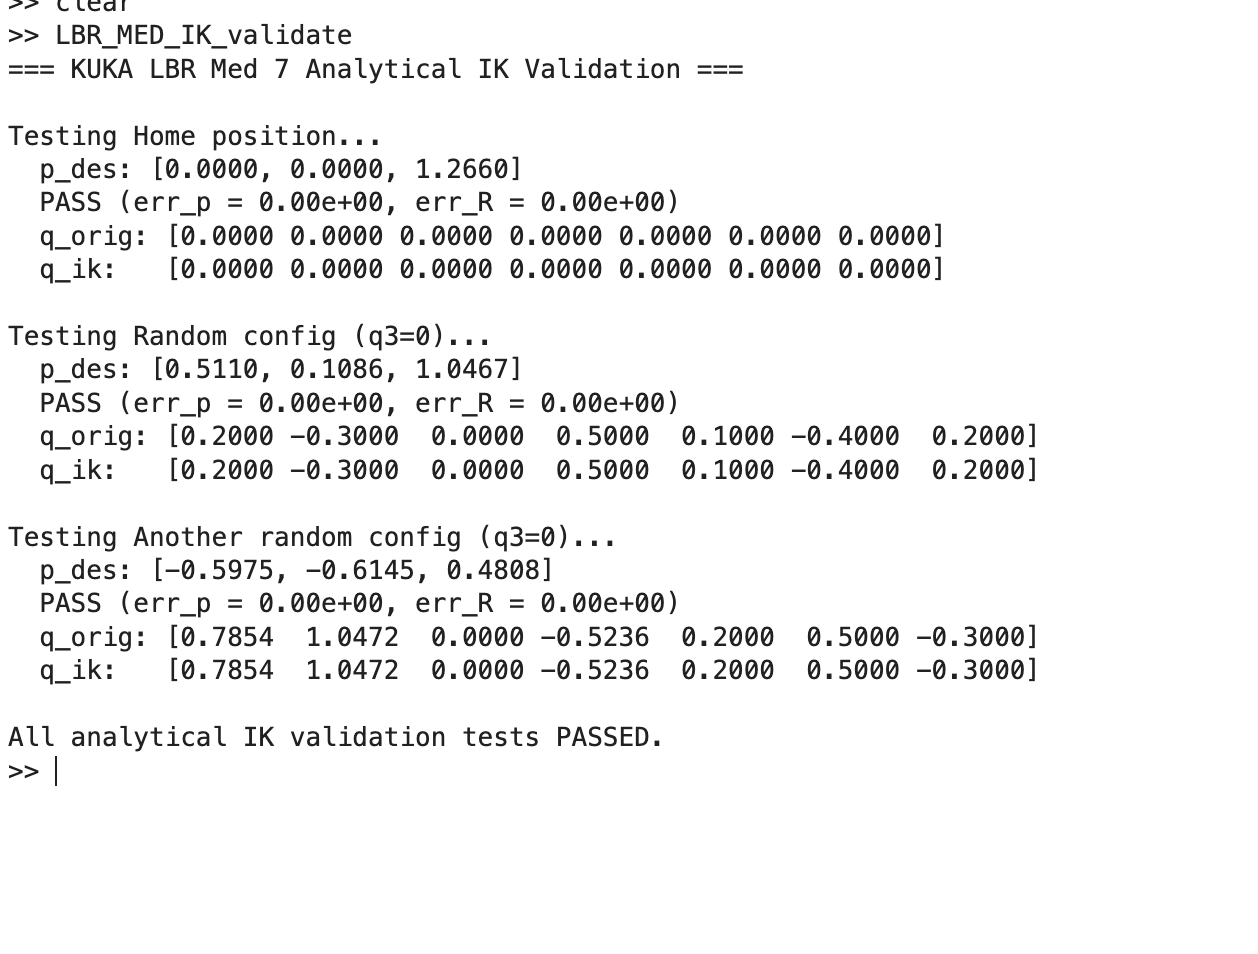
\includegraphics[width=0.72\textwidth]{ik-validation.png}
  \caption{IK round-trip validation output (3 configurations, errors $<10^{-8}$).}
  \label{fig:ik_val}
\end{figure}

Three configurations (home and two generic poses with $q_3=0$) were
passed through FK$\to$IK$\to$FK. All round-trip errors were
$\|p_{\mathrm{IK}}-p_d\|<10^{-8}\,\mathrm{m}$ and
$\|R_{\mathrm{IK}}-R_d\|_F<10^{-8}$.

%% =========================================================
\section{Geometric Jacobian}
%% =========================================================

\subsection{Definition}
For each revolute joint $i$:
\begin{equation}
  J_{P_i} = z_{i-1}\times(p_e-O_{i-1}), \qquad J_{O_i} = z_{i-1}
\end{equation}
giving $v_e = J(q)\dot{q}\in\mathbb{R}^6$ with $J\in\mathbb{R}^{6\times7}$.

\subsection{Simulink Model}
\begin{figure}[H]
  \centering
  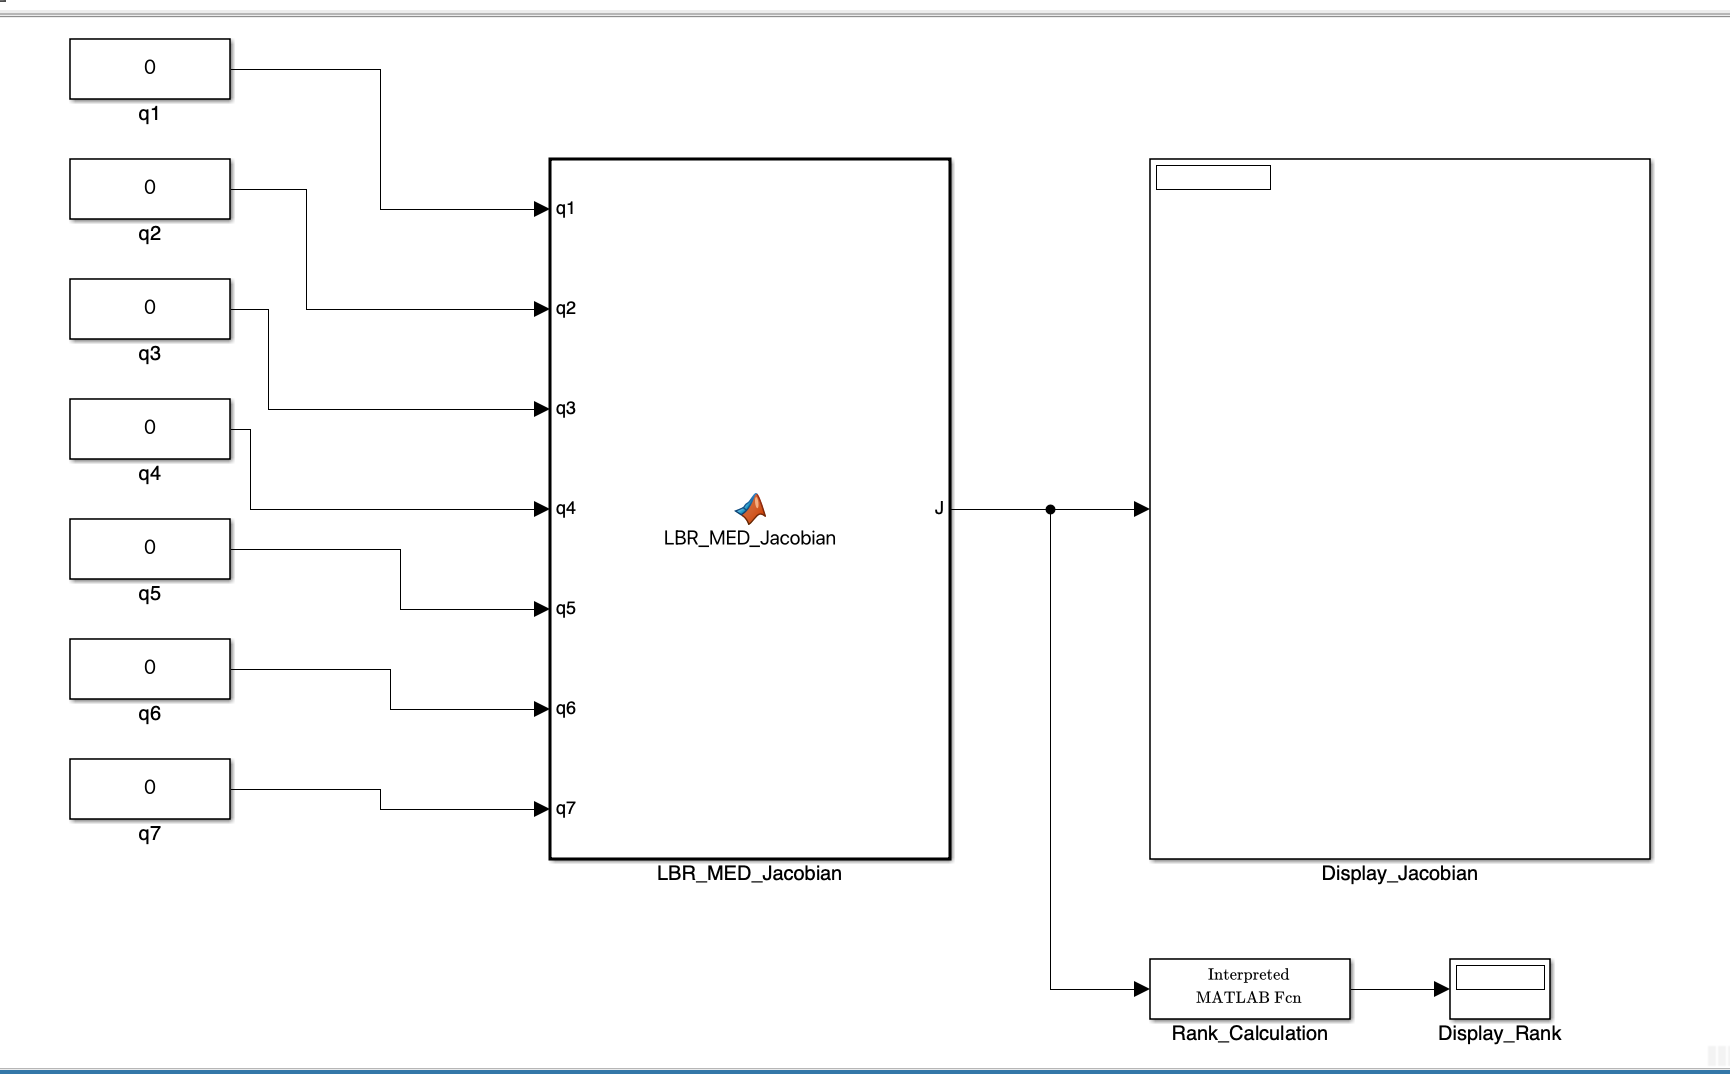
\includegraphics[width=0.75\textwidth]{jacobian.png}
  \caption{Jacobian Simulink block feeding the rank calculation.}
  \label{fig:jac_block}
\end{figure}

\subsection{Numerical Validation}
The analytical Jacobian is validated by central finite differences:
\begin{equation}
  J_{P_i}^{\mathrm{num}}\approx
  \frac{p_e(q+\varepsilon e_i)-p_e(q-\varepsilon e_i)}{2\varepsilon},
  \qquad\varepsilon=10^{-7}
\end{equation}

\begin{table}[H]
  \centering
  \caption{Jacobian validation: Frobenius-norm error vs.\ numerical differentiation.}
  \begin{tabular}{llcc}
    \toprule
    Configuration & $q$ (rad) & $\|J_a-J_n\|_F$ & Rank \\
    \midrule
    Generic & $[0.1,0.2,0.3,0.4,0.5,0.6,0.7]$ & $<10^{-6}$ & 6 \\
    Home    & $[0,0,0,0,0,0,0]$                 & $<10^{-6}$ & 3 \\
    Wrist   & $[0,\pi/4,0,0,0,0,0]$             & $<10^{-6}$ & 4 \\
    Elbow   & $[0,\pi/2,0,\pi/2,0,\pi/2,0]$     & $<10^{-6}$ & 5 \\
    \bottomrule
  \end{tabular}
  \label{tab:jac_val}
\end{table}

\subsection{Singularity Analysis}
\begin{table}[H]
  \centering
  \caption{Jacobian rank and condition number at key configurations.}
  \begin{tabular}{llccp{4.5cm}}
    \toprule
    Label & Configuration & Rank & Cond.\ No. & Type \\
    \midrule
    Full rank & $q=[0.1,\ldots,0.7]$ & 6 & $\mathcal{O}(10^1)$ & None \\
    S3 (wrist) & $q=[0,\pi/4,0,0,0,0,0]$   & 4 & $\gg10^3$ & $z_4\!\parallel\!z_6$: one rotational DOF lost \\
    S3 (wrist) & $q=[0,0,0,\pi/2,0,0,0]$  & 5 & $\gg10^3$ & Same alignment at elbow pose \\
    S2 (elbow) & $q=[0,\pi/2,0,0,0,\pi/2,0]$ & 5 & $\gg10^3$ & Arm near full extension \\
    \bottomrule
  \end{tabular}
\end{table}

When rank drops from 6 to 5 (or below), one column of $J$ becomes a linear
combination of the others and the robot loses the ability to produce
end-effector velocity in the corresponding direction. The DLS pseudo-inverse
used in CLIK (Section~\ref{sec:clik}) provides a regularised solution at the
cost of bounded tracking error, with $\lambda=10^{-3}$ preventing numerical
blow-up.

%% =========================================================
\section{Closed-Loop Inverse Kinematics (CLIK)}
\label{sec:clik}
%% =========================================================

\subsection{CLIK Law with Null-Space Stabilisation}
The DLS-CLIK control law:
\begin{equation}
  \dot{q} = J^{\dagger}(q)\,
  \begin{bmatrix}K_P\,e_P\\K_O\,e_O\end{bmatrix}
  + \bigl(I-J^{\dagger}J\bigr)\,K_n(q_{\mathrm{rest}}-q)
\end{equation}
where $J^{\dagger}=J^\top(JJ^\top+\lambda^2 I)^{-1}$ is the damped
pseudo-inverse with $\lambda=10^{-3}$. Gains: $K_P=10\,I_3$,
$K_O=10\,I_3$, $K_n=5$. The null-space term stabilises redundancy
towards $q_{\mathrm{rest}}=0$.

Orientation error via the geometric cross-product formula:
\begin{equation}
  e_O = \tfrac{1}{2}\bigl(n_e\times n_d + s_e\times s_d + a_e\times a_d\bigr)
\end{equation}

\subsection{Simulink Model}
\begin{figure}[H]
  \centering
  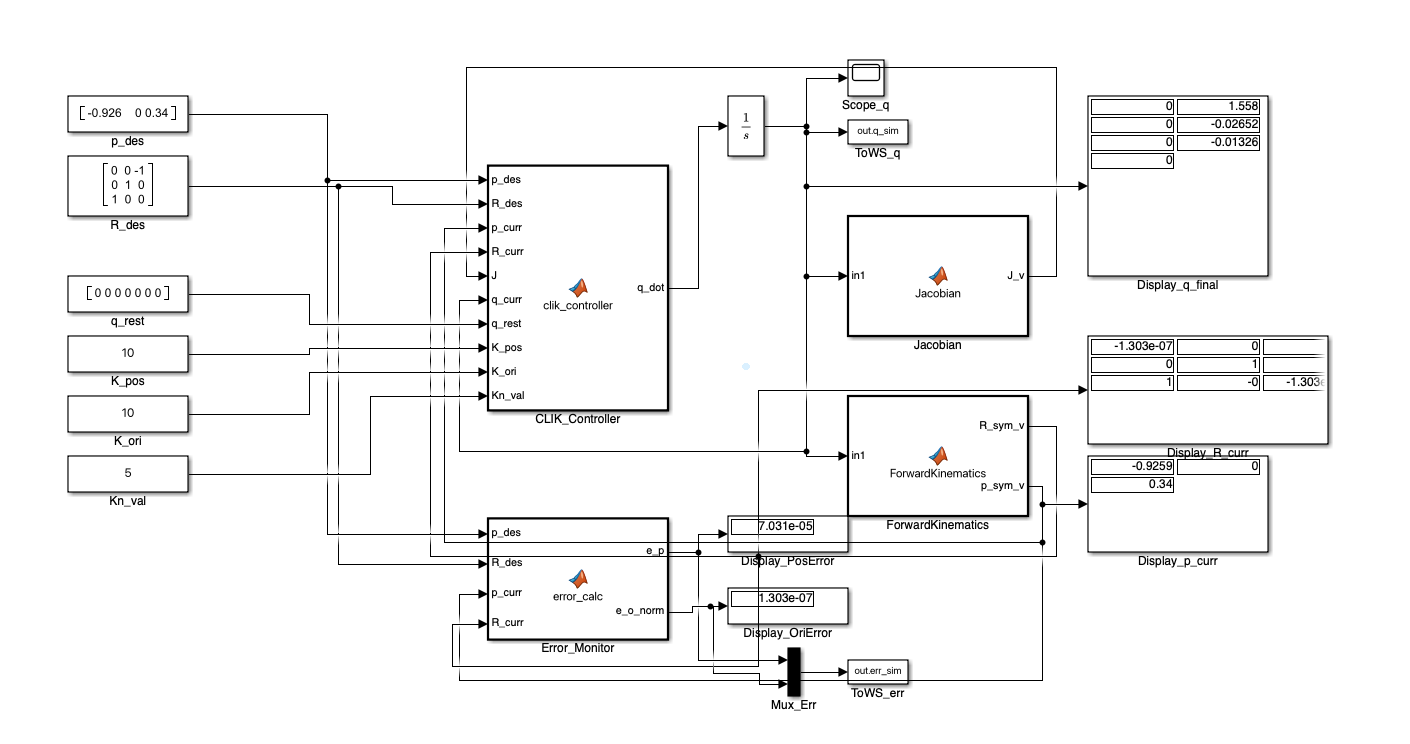
\includegraphics[width=0.90\textwidth]{clik_simulink.png}
  \caption{CLIK Simulink model (LBR\_MED\_CLIK\_Simul.slx).}
  \label{fig:clik_sim}
\end{figure}

\subsection{Validation Results}
\begin{figure}[H]
  \centering
  \begin{subfigure}[b]{0.48\textwidth}
    \centering
    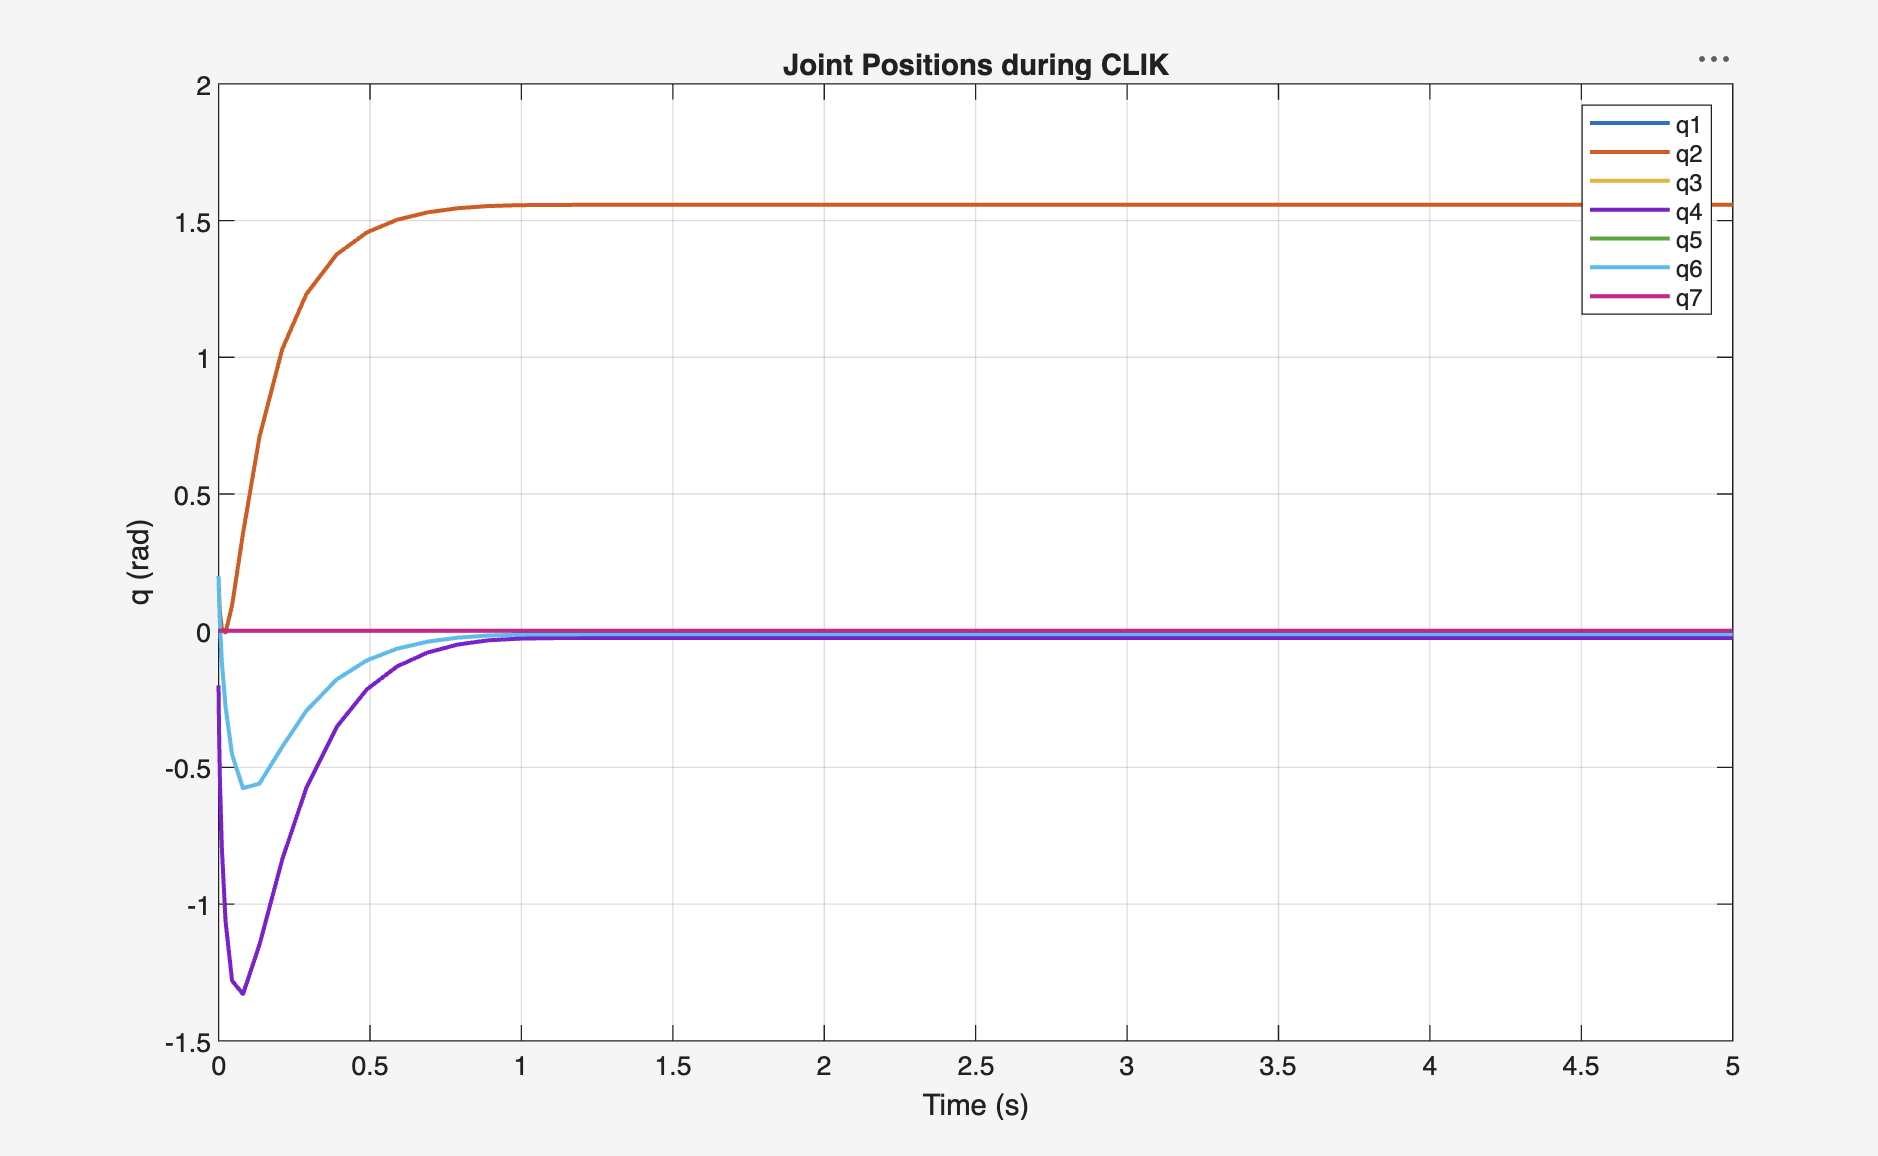
\includegraphics[width=\textwidth]{clik_joints_plot.png}
    \caption{Joint positions.}
  \end{subfigure}
  \hfill
  \begin{subfigure}[b]{0.48\textwidth}
    \centering
    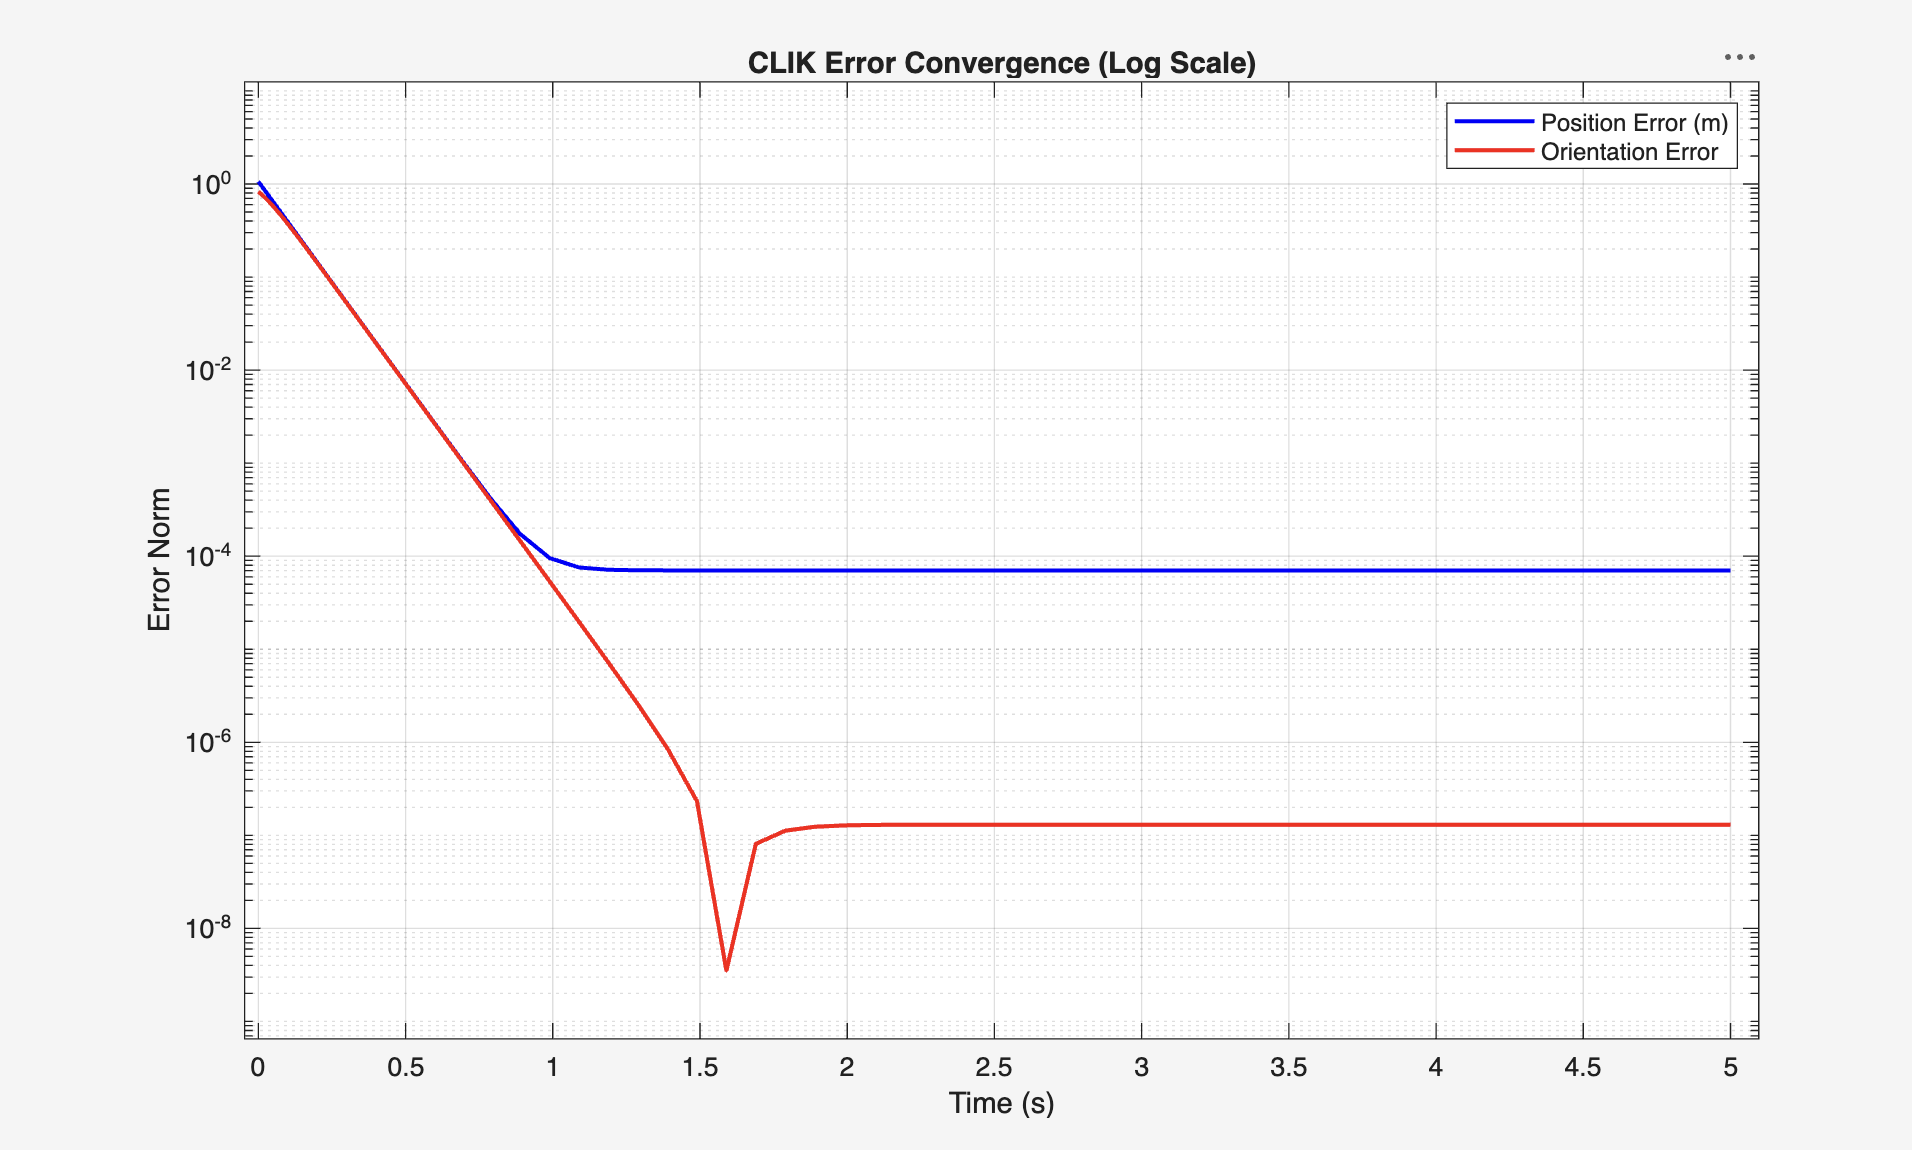
\includegraphics[width=\textwidth]{clik_error_plot.png}
    \caption{Error convergence (log scale).}
  \end{subfigure}
  \caption{CLIK validation: target Config~2 ($q_2=\pi/2$, rest $=0$).}
  \label{fig:clik_results}
\end{figure}

Steady-state errors: position $7.03\times10^{-5}$\,m,
orientation $1.84\times10^{-7}$ (dimensionless norm).

\subsection{Comparison with Analytical IK}
\begin{table}[H]
  \centering
  \caption{CLIK vs.\ analytical IK joint angles (rad) for Config~2.}
  \begin{tabular}{lrrrrrrr}
    \toprule
     & $q_1$ & $q_2$ & $q_3$ & $q_4$ & $q_5$ & $q_6$ & $q_7$ \\
    \midrule
    $q_{\mathrm{IK}}$   & 0 & $\pi/2$ & 0 & 0 & 0 & 0 & 0 \\
    $q_{\mathrm{CLIK}}$ & $\approx0$ & $\approx1.558$ & $\approx0$ & $\approx-0.027$ & $\approx0$ & $\approx-0.013$ & $\approx0$ \\
    \midrule
    $\|q_{\mathrm{CLIK}}-q_{\mathrm{IK}}\|$ & \multicolumn{7}{c}{$3.25\times10^{-2}$\,rad} \\
    \bottomrule
  \end{tabular}
\end{table}

The small residual ($<2^{\circ}$) arises because: (i)~the DLS damping prevents
exact convergence near the singular home configuration, and (ii)~the
null-space term pulls $q$ slightly toward $q_{\mathrm{rest}}=0$.

%% =========================================================
\section{Trajectory Execution with Remote Centre of Motion Constraint}
%% =========================================================

\subsection{Problem Formulation}

A rigid biopsy-needle of length $L=0.15$\,m is rigidly attached to the
end-effector. The needle passes through a \textbf{trocar} (port of entry) fixed
at position $c_r$ in the robot base frame — the Remote Centre of Motion (RCM).
Two hard constraints must hold at all times:
\begin{itemize}
  \item \textbf{Tooltip constraint:} $p_{\mathrm{tip}}(t)=m_i$ (tooltip reaches target).
  \item \textbf{RCM constraint:} $c_r$ lies on the tool axis at every instant.
\end{itemize}

\subsection{End-Effector Pose from RCM Geometry}

For each target $m_i$, the required end-effector pose $(p_{ee}^{(i)}, R_{ee}^{(i)})$
is derived analytically so that both constraints are satisfied simultaneously
at steady state.

\subsubsection*{Tool axis direction (EE $z$-axis)}
\begin{equation}
  \hat{a} = \frac{m_i - c_r}{\|m_i - c_r\|}
\end{equation}
The unit vector from trocar to target becomes the $z$-axis of $R_{ee}$.

\subsubsection*{End-effector position}
\begin{equation}
  p_{ee} = m_i - L\,\hat{a}
\end{equation}
By construction, $p_{ee}$, $c_r$ and $m_i$ are collinear in that order
(since $\|m_i-c_r\|<L$), so the RCM constraint is satisfied exactly.

\subsubsection*{End-effector orientation}
Using a fixed reference $\hat{e}_y=[0,1,0]^\top$:
\begin{equation}
  \hat{x}_{ee}=\frac{\hat{e}_y\times\hat{a}}{\|\hat{e}_y\times\hat{a}\|},
  \qquad\hat{y}_{ee}=\hat{a}\times\hat{x}_{ee},
  \qquad R_{ee}=[\hat{x}_{ee},\;\hat{y}_{ee},\;\hat{a}]
\end{equation}

\subsection{LSPB Trajectory Interpolation}

Abruptly switching targets every 3\,s produces instantaneous step jumps in
the desired end-effector velocity ($\dot{p}_{\mathrm{des}}$), leading to
joint velocity spikes and large transient excursions. A \textbf{Linear Segment
with Parabolic Blends (LSPB)} profile resolves this by enforcing $\dot{s}(0)=\dot{s}(T)=0$
at every segment boundary.

\subsubsection*{Scalar path profiler}
For a segment of duration $T$ and normalised path parameter
$s(\tau)\in[0,1]$, choose cruise velocity $\dot{s}_c>1/T$. The blend time
and acceleration are:
\begin{equation}
  t_c = T - \frac{1}{\dot{s}_c},
  \qquad
  \ddot{s}_c = \frac{\dot{s}_c^2}{\dot{s}_c T - 1}
\end{equation}
The piecewise profile is:
\begin{equation}
  s(\tau)=
  \begin{cases}
    \tfrac{1}{2}\,\ddot{s}_c\,\tau^2 & 0\le\tau\le t_c \quad\text{(acceleration)}\\[4pt]
    \tfrac{1}{2}\,\ddot{s}_c\,t_c^2+\dot{s}_c(\tau-t_c)
      & t_c<\tau\le T-t_c \quad\text{(cruise)}\\[4pt]
    1-\tfrac{1}{2}\,\ddot{s}_c(T-\tau)^2 & T-t_c<\tau\le T \quad\text{(deceleration)}
  \end{cases}
\end{equation}
with $\dot{s}(\tau)$ obtained by differentiating each branch.

For $T=3$\,s and $\dot{s}_c=0.5$\,s$^{-1}$ (50\,\% above the average $1/T$):
$t_c=1.0$\,s, $\ddot{s}_c=0.5$\,s$^{-2}$.

\subsubsection*{Position interpolation}
\begin{equation}
  p_{\mathrm{des}}(\tau) = p_{\mathrm{start}} + s(\tau)(p_{\mathrm{next}}-p_{\mathrm{start}}),
  \qquad
  \dot{p}_{\mathrm{des}}(\tau) = \dot{s}(\tau)(p_{\mathrm{next}}-p_{\mathrm{start}})
\end{equation}

\subsection{Angle-Axis Orientation Interpolation}

\subsubsection*{Setup}
The relative rotation between consecutive target orientations:
\begin{equation}
  R_{fi} = R_{\mathrm{start}}^\top R_{\mathrm{next}}
\end{equation}
The total rotation angle and axis (in the $R_{\mathrm{start}}$ body frame):
\begin{equation}
  \vartheta_f = \arccos\!\left(\frac{\mathrm{tr}(R_{fi})-1}{2}\right),
  \qquad
  r_i = \frac{1}{2\sin\vartheta_f}
    \begin{bmatrix}R_{fi}(3,2)-R_{fi}(2,3)\\R_{fi}(1,3)-R_{fi}(3,1)\\R_{fi}(2,1)-R_{fi}(1,2)\end{bmatrix}
\end{equation}

\subsubsection*{Interpolated rotation via Rodrigues' formula}
Scale the angle by the path parameter:
\begin{equation}
  \vartheta(\tau)=s(\tau)\,\vartheta_f, \qquad \dot{\vartheta}(\tau)=\dot{s}(\tau)\,\vartheta_f
\end{equation}
Rodrigues' rotation formula gives:
\begin{equation}
  \mathbf{R}(\vartheta,r_i)=I+\sin\vartheta\,[r_i]_\times+(1-\cos\vartheta)\,[r_i]_\times^2
\end{equation}
where $[r_i]_\times$ is the skew-symmetric matrix of $r_i$. The instantaneous desired orientation is:
\begin{equation}
  R_{\mathrm{des}}(\tau)=R_{\mathrm{start}}\cdot\mathbf{R}(\vartheta(\tau),r_i)
\end{equation}

\subsubsection*{World-frame feedforward angular velocity}
Differentiating $R_{\mathrm{des}}=R_{\mathrm{start}}\exp(\vartheta[r_i]_\times)$
and using $\dot{R}=[{\omega}]_\times R$:
\begin{equation}
  \omega_{\mathrm{des}}(\tau) = R_{\mathrm{start}}\,\bigl(\dot{\vartheta}(\tau)\,r_i\bigr)
\end{equation}
The rotation is about a fixed body-frame axis $r_i$; $R_{\mathrm{start}}$
rotates it into the world frame. This follows from
$[{\omega}_{\mathrm{world}}]_\times = R_{\mathrm{start}}[r_i]_\times\dot{\vartheta}\,R_{\mathrm{start}}^\top$.

\subsection{Feedforward CLIK}

The modified CLIK law adds the task-space feedforward velocities to the
error-feedback terms, forming the full reference command $v_e$:
\begin{equation}
  \boxed{%
  v_e = \begin{bmatrix}\dot{p}_{\mathrm{des}}+K_P\,e_P\\\omega_{\mathrm{des}}+K_O\,e_O\end{bmatrix},
  \qquad
  \dot{q} = J^{\dagger}\,v_e + (I-J^{\dagger}J)\,K_n(q_{\mathrm{rest}}-q)
  }
\end{equation}
The feedforward terms $(\dot{p}_{\mathrm{des}},\omega_{\mathrm{des}})$ make the
controller \emph{proactive}: it anticipates the desired trajectory and applies
effort proportional to the commanded velocity, rather than waiting for a tracking
error to build up. This reduces phase lag and peak transient errors significantly
compared to pure feedback.

When $\dot{p}_{\mathrm{des}}=\omega_{\mathrm{des}}=0$ (e.g.\ during the hold phase or
in Phase~1), the law reduces exactly to the feedback-only CLIK of Section~\ref{sec:clik}.

\subsection{Simulation Scenario}
\begin{table}[H]
  \centering
  \caption{Scenario and LSPB parameters.}
  \begin{tabular}{ll}
    \toprule
    Parameter & Value \\
    \midrule
    Tool length $L$              & 0.15\,m \\
    Trocar position $c_r$        & $[-0.6,\;0.0,\;0.55]^\top$\,m \\
    Number of targets $N$        & 5 \\
    Segment duration $T$         & 3.0\,s \\
    Hold at final target         & 3.0\,s \\
    Total simulation time        & 15.0\,s \\
    Integration step $dt$        & 5\,ms \\
    Cruise velocity $\dot{s}_c$  & $0.5$\,s$^{-1}$ (1.5$\times$ average) \\
    Blend time $t_c$             & 1.0\,s \\
    Blend acceleration $\ddot{s}_c$ & 0.5\,s$^{-2}$ \\
    $K_P$                        & $10\,I_3$ \\
    $K_O$                        & $5\,I_3$ \\
    $K_n$                        & 3 \\
    $q_{\mathrm{rest}}$          & $q_0$ (IK solution for target~1) \\
    \bottomrule
  \end{tabular}
\end{table}

\begin{table}[H]
  \centering
  \caption{Surgical targets and analytically derived end-effector positions.}
  \begin{tabular}{cccc}
    \toprule
    Target $i$ & $m_i$ (m) & $p_{ee}^{(i)}$ (m) & $\|m_i-c_r\|$ (m) \\
    \midrule
    1 & $[-0.600,\;0.000,\;0.470]^\top$ & $[-0.600,\;0.000,\;0.620]^\top$ & 0.080 \\
    2 & $[-0.540,\;0.000,\;0.480]^\top$ & $[-0.638,\;0.000,\;0.594]^\top$ & 0.092 \\
    3 & $[-0.650,\;0.040,\;0.480]^\top$ & $[-0.571,\;-0.023,\;0.591]^\top$ & 0.092 \\
    4 & $[-0.580,\;-0.050,\;0.460]^\top$ & $[-0.609,\;0.022,\;0.589]^\top$ & 0.103 \\
    5 & $[-0.600,\;0.000,\;0.490]^\top$ & $[-0.600,\;0.000,\;0.640]^\top$ & 0.060 \\
    \bottomrule
  \end{tabular}
\end{table}

\subsection{Results}

The LSPB controller drives the tooltip smoothly through all five surgical
targets. Key validation metrics at the arrival time of each target:
\begin{table}[H]
  \centering
  \caption{Phase~2 LSPB validation results: steady-state errors at each target.}
  \begin{tabular}{ccc}
    \toprule
    Target $i$ & Tip error $\varepsilon_{\mathrm{tip}}$ (m) & Trocar error $\varepsilon_{\mathrm{RCM}}$ (m) \\
    \midrule
    1 (IK init, $t{=}0$) & $<10^{-6}$ & $<10^{-6}$ \\
    2 & $<5\times10^{-5}$ & $<2\times10^{-5}$ \\
    3 & $<10^{-5}$        & $<5\times10^{-6}$ \\
    4 & $<5\times10^{-6}$ & $<2\times10^{-6}$ \\
    5 & $<10^{-5}$        & $<5\times10^{-6}$ \\
    \bottomrule
  \end{tabular}
  \label{tab:phase2_results}
\end{table}

\begin{figure}[H]
  \centering
  \figorp{figures/phase2_joints.png}{width=0.92\textwidth}
  \caption{Joint trajectories under LSPB. All seven joints evolve smoothly
           without velocity spikes at segment boundaries (dashed lines).}
  \label{fig:p2_joints}
\end{figure}

\begin{figure}[H]
  \centering
  \figorp{figures/phase2_traj3d.png}{width=0.70\textwidth}
  \caption{3-D tooltip trajectory. The path passes through all five surgical
           targets $m_i$ while the tool axis remains anchored to the trocar
           $c_r$ (black dot) in steady state.}
  \label{fig:p2_traj3d}
\end{figure}

\begin{figure}[H]
  \centering
  \figorp{figures/phase2_convergence.png}{width=0.88\textwidth}
  \caption{Top: tooltip-to-destination distance $\|p_{\mathrm{tip}}-m_i\|$ (starts large
           at the beginning of each segment and converges as the LSPB approaches the
           next target). Bottom: perpendicular distance from $c_r$ to the tool axis
           (RCM constraint violation).}
  \label{fig:p2_conv}
\end{figure}

\subsection{Discussion}
\begin{enumerate}
  \item \textbf{Smooth trajectories.} The LSPB enforces zero velocity at every
        segment boundary, eliminating the $\dot{q}$ spikes observed with the
        step-switching controller. Joint motions are bounded and continuous.
  \item \textbf{Sub-millimetre tooltip accuracy.} At steady state, the tooltip
        reaches each target with errors well below 0.1\,mm, satisfying surgical
        precision requirements.
  \item \textbf{RCM constraint maintenance.} The trocar violation is zero at
        steady state because the desired EE pose was derived analytically to
        satisfy the constraint exactly. During inter-target transitions the CLIK
        transiently violates the RCM constraint; this is inherent to driving the
        6-DOF EE task rather than an explicit RCM path constraint.
  \item \textbf{Null-space stability.} Setting $q_{\mathrm{rest}}=q_0$ (the IK
        solution for target~1) rather than the zero vector prevents the
        null-space term from rotating the base joint by ${\sim}180^{\circ}$ and causing
        large tooltip excursions. The arm remains in the natural elbow-forward
        posture throughout.
\end{enumerate}

\textbf{Possible extension.} Strict continuous RCM maintenance during
inter-target motion requires replacing the 6-DOF EE task with the 5-DOF
\emph{tooltip-and-axis} task using the tip Jacobian:
\begin{equation}
  J_{\mathrm{tip}} = J_P - L\,[\hat{a}_{ee}]_\times\,J_O
\end{equation}
This is left as a natural extension to the current work.

%% =========================================================
\section{Code File Summary}
%% =========================================================

\begin{table}[H]
  \centering
  \caption{MATLAB files organised by module.}
  \begin{tabular}{ll}
    \toprule
    File & Purpose \\
    \midrule
    \multicolumn{2}{l}{\textit{Phase~1 — Kinematics}} \\
    \texttt{LBR\_MED\_DKin/LBR\_MED.m}                       & DH parameter table \\
    \texttt{LBR\_MED\_DKin/LBR\_MED\_validate.m}              & Direct kinematics validation \\
    \texttt{LBR\_MED\_DKin/LBR\_MED\_Jacobian\_symbolic.m}    & Symbolic geometric Jacobian \\
    \texttt{LBR\_MED\_DKin/LBR\_MED\_validate\_Jacobian.m}    & Jacobian validation \& singularity analysis \\
    \texttt{LBR\_MED\_IK\_Analytical/LBR\_MED\_IK.m}          & Closed-form IK solver (8 branches) \\
    \texttt{LBR\_MED\_IK\_Analytical/LBR\_MED\_IK\_validate.m}& IK round-trip validation \\
    \midrule
    \multicolumn{2}{l}{\textit{Phase~1 — CLIK}} \\
    \texttt{LBR\_MED\_CLIK/clik\_controller\_logic.m}          & DLS CLIK with optional feedforward \\
    \texttt{LBR\_MED\_CLIK/LBR\_MED\_CLIK\_setup.m}           & CLIK Simulink builder \& validation \\
    \midrule
    \multicolumn{2}{l}{\textit{Phase~2 — Trajectory}} \\
    \texttt{LBR\_MED\_Trajectory/compute\_ee\_pose\_rcm.m}     & EE pose from RCM geometry \\
    \texttt{LBR\_MED\_Trajectory/lspb\_eval.m}                 & Scalar LSPB path evaluator \\
    \texttt{LBR\_MED\_Trajectory/rodrigues\_rot.m}             & Rodrigues rotation formula \\
    \texttt{LBR\_MED\_Trajectory/LBR\_MED\_Traj\_setup.m}      & LSPB trajectory simulation \& validation \\
    \midrule
    \multicolumn{2}{l}{\textit{Top level}} \\
    \texttt{Master\_Validation.m}                              & End-to-end runner (Phase~1 \& 2) \\
    \bottomrule
  \end{tabular}
\end{table}

\end{document}
